\documentclass{beamer}

\usepackage[utf8]{inputenc}

\title[SymEngine \hspace{14em}\insertframenumber/
\inserttotalframenumber]{SymEngine: \\A Fast Symbolic Manipulation Library}

\usepackage{graphicx}
\graphicspath{ {images/} }


\author[O. Čertík, I. Fernando, ...]{Ondřej Čertík, Isuru Fernando, Thilina Rathnayake, Abhinav Agarwal, Sumith Kulal, Abinash Meher, Rajith Vidanaarachchi, Shikhar Jaiswal, Ranjith Kumar}

\begin{document}


\begin{frame}
\maketitle
\end{frame}


\begin{frame}{Outline}
\begin{block}{SymEngine}
\begin{itemize}
\item Introduction
\item Features
\item Demo (Python, Ruby, Julia)
\item Why C++, how to write safe code
\item Internals of SymEngine
\item SymEngine and SymEngine.py
\item Roadmap for using SymEngine in SymPy
\item Roadmap for using SymEngine in Sage
\item Roadmap for using SymEngine in PyDy
\item Benchmarks
\end{itemize}
\end{block}
\end{frame}


\begin{frame}
\frametitle{Introduction}
\framesubtitle{About SymEngine}
\begin{itemize}
\item Symbolic manipulation library written in C++
\item Thin wrappers to Python, Ruby, Julia, C and Haskell
\item MIT licensed
\item Started in 2012
\item 46 contributors
\item Runs on Linux (GCC, Clang, Intel), OS X (GCC, Clang), Windows (MSVC,
    MinGW, MinGW-w64)
\item Part of the SymPy organization, but the C++ library is Python independent
\end{itemize}
\end{frame}


\begin{frame}
\frametitle{Introduction}
\framesubtitle{Goals}
\begin{itemize}
\item Be the fastest symbolic manipulation library (open-source or commercial)
\item Serve as the core for SymPy and Sage, optionaly supporting PyDy
\item Serve as the default symbolic manipulation library in other languages
    thanks to thin wrappers (Python, Ruby, Julia, C and Haskell)
\end{itemize}
\end{frame}


\begin{frame}
\frametitle{Choice of Language}
\begin{block}{Problem}
SymPy speed is sometimes insufficient
\begin{itemize}
\item Handling of very large expressions
\item Large calculations using small/medium size expressions
\end{itemize}
\end{block}

\begin{block}{Let's Fix That}
\begin{itemize}
\item We tried: pure Python/PyPy, Cython, C, ...
\item Investigated Julia, Rust, Scala, Javascript, ...
\item Chose C++
\end{itemize}
\end{block}
\end{frame}




\begin{frame}
\frametitle{Current Features}
\begin{itemize}
    \item Core (Symbols, +, -, *, /, **)
    \item Elementary Functions (sin, cos, gamma, erf)
    \item Number Theory
    \item Differentiation, Substitution
    \item Matrices and Sets
    \item Polynomials (Piranha, Flint)
    \item Series Expansion
    \item Solvers (Polynomial and Trigonometric)
    \item Printing, Parsing and Code Generation
    \item Numeric Evaluation (Double and Arbitrary Precision)
\end{itemize}
\end{frame}

\begin{frame}
\frametitle{Demo}
{\Large\bf Demo Time}
\end{frame}


\begin{frame}
\frametitle{Why Pure C++}
\begin{itemize}
\item Fast in Release mode, but safe in Debug mode
\item Compiler helps (not as good as Scala or Haskell, but much better than
    Python)
\item Just one language to learn, thus easy to maintain (as opposed to several
    intertwined layers such as C + Cython + Python)
\item Thin wrappers (that core developers do not need to maintain), all functionality in C++
\item Easier to create bindings to other languages like Python, Julia, Ruby and Haskell
\end{itemize}
\end{frame}

\begin{frame}
\frametitle{Why Pure C++: Fast in Release Mode}
\begin{itemize}
    \item Allows direct memory handling (allocation, deallocation, access)
    \item Allows to tweak how and when things are done
    \item It is possible to go to bare metal
    \item Allows reasonably high level abstractions (simple, maintainable
        code)
\end{itemize}
\end{frame}

\begin{frame}
\frametitle{Why Pure C++: Safe in Debug Mode}
\begin{itemize}
    \item Reference counted pointers \texttt{Teuchos::RCP} (from Trilinos)
    \item Checks for dangling and null pointers (exception is raised)
    \item No raw pointers/references (use \texttt{Ptr} and \texttt{RCP})
    \item Use a safe subset of C++
    \item Few other rules, e.g. how to use \texttt{Ptr} and \texttt{RCP}
          properly
    \item Possible to visually verify in a PR (pull request) review
    \item Hopefully eventually there are plugins to Clang to check
        automatically (since the rules are simple and static)
    \item As fast as raw pointers in Release mode (but it could segfault)
\end{itemize}
    Conclusion: the code cannot segfault or have undefined behavior in Debug
    mode --- always get an exception at runtime, or a compile error.
\end{frame}


\begin{frame}
\frametitle{Internals of SymEngine}
\framesubtitle{How Add Class Works}
\begin{itemize}
    \item Add stores the various algebraic terms in a dictionary as variable-coefficient 
        pairs, while separately storing the constant term of the expression
    \item Add uses \texttt{std::unordered\_map} (hashtable) for the dictionary
        \begin{itemize}
            \item $2xy^2+3x^2y + 5\to \{xy^2: 2, x^2y: 3\}; coeff=5 $
        \end{itemize}
    \item Each object is reference counted (RCP), hence very fast implementation in
        Release mode
\end{itemize}
\end{frame}


\begin{frame}
\frametitle{Internals of SymEngine}
\framesubtitle{How Mul Class Works}
\begin{itemize}
    \item Mul stores the various algebraic terms in a dictionary as base-exponent 
        pairs, while separately storing the constant coefficient of the expression
    \item Mul uses \texttt{std::map} (red-black tree)
        \begin{itemize}
            \item $2 xy^2 \to \{x: 1, y:2\}; coeff=2$
        \end{itemize}
    \item Each object is, like in the case of Add class, reference counted (RCP)
\end{itemize}
\end{frame}


\begin{frame}
\frametitle{Internals of SymEngine}
\framesubtitle{How Pow Class Works}
\begin{itemize}
    \item Pow just stores the base and exponent as individual RCP objects, no dictionaries are used for storage
        \begin{itemize}
            \item $ x^5 \to base=x; coeff=5$
        \end{itemize} 
\end{itemize}
\end{frame}


\begin{frame}
\frametitle{Internals of SymEngine}
\framesubtitle{Extensibility using Visitor Pattern}
\begin{itemize}
    \item All algorithms implemented using visitor pattern
    \item Algorithm is implemented in its own file, separate from the core
    \item Two virtual function calls (can be implemented in third party code or
        user code)
    \item Special version with just one virtual function call (faster, but must
        be compiled as part of the SymEngine source code)
    \item The speed difference between the two is minor for practical purposes
\end{itemize}
\end{frame}


\begin{frame}[fragile]
\frametitle{SymEngine and SymEngine.py}
\framesubtitle{Designing The Interface}
\begin{itemize}
    \item SymEngine.py uses Cython's native support for C++ constructs.
    \item Uses Cython's $libcpp$ module for importing $bool$, $string$, $map$,
        $vector$ and $pair$ data types.
    \item Declares $set$, $multiset$ and $unordered\_map$ directly from C++'s 
        $<set>$ module, as Cython's $libcpp.set$ does not support multi-template 
        arguments to any of them.
    \begin{verbatim}
    cdef extern from "<set>" namespace "std":
        cdef cppclass set[T, U]:
    \end{verbatim}
\end{itemize}
\end{frame}


\begin{frame}[fragile]
\frametitle{SymEngine and SymEngine.py}
\framesubtitle{Designing The Interface}
\begin{itemize}
    \item Additionally, maintains .pxd files with cdef extern from blocks and (if existing)
        the C++ namespace name:
    \begin{verbatim}
    cdef extern from "<symengine/symbol.h>" namespace 
    "SymEngine":
    \end{verbatim}
\item In these blocks, we declare SymEngine's classes as cdef cppclass blocks:
    \begin{verbatim}
    cdef cppclass Symbol(Basic):
    \end{verbatim}
\item And then declare SymEngine's public names (variables, methods and constructors):
    \begin{verbatim}
    Symbol(string name) nogil
    string get_name() nogil
    \end{verbatim}
\end{itemize}
\end{frame}


\begin{frame}
\frametitle{SymEngine and SymEngine.py}
\framesubtitle{Working With SymEngine's Data Types}
\begin{itemize}
    \item Cython classes implemented for data types available in SymEngine, and Python
        classes for types currently unavailable.
    \item As soon as a class object is called, a SymEngine equivalent object is created
        and passed to a dedicated function ($c2py$).
    \item The function takes the object and returns the corresponding Cython
        or Python counterpart for usage.
    \item Conversely, another dedicated function ($sympy2symengine$) takes a Python object
        and returns the SymEngine equivalent.
\end{itemize}
\end{frame}


\begin{frame}
\frametitle{SymEngine and SymEngine.py}
\framesubtitle{Testing The Interface}
\begin{itemize}
    \item Since specific classes are created for each data type, the functionalities
        can be directly called, just as in the case of SymPy.
    \item Most of the test cases derive directly from SymPy's test suite for filtering
        out inconsistencies and finding the fundamental differences.
\end{itemize}
\end{frame}


\begin{frame}[fragile]
\frametitle{SymPy, SymEngine and SymEngine.py}
\framesubtitle{Using SymEngine in SymPy}
\begin{itemize}
\item
SymEngine will convert any SymPy object to a corresponding SymEngine object before doing any operation

\begin{verbatim}
>>> from symengine import symbols, Add
>>> import sympy
>>> x = symbols("x")
>>> y = sympy.symbols("y")
>>> x + y
x + y
>>> type(x+y)
<type 'symengine.lib.symengine_wrapper.Add'>
\end{verbatim}
\item
What if there is no corresponding SymEngine object?
\end{itemize}
\end{frame}


\begin{frame}[fragile]
\frametitle{SymPy, SymEngine and SymEngine.py}
\framesubtitle{Using SymEngine in SymPy}
\begin{itemize}
\item
SymEngine will keep a reference to a SymPy object if there is no corresponding SymEngine object using Python/C API.
SymEngine will use Python callbacks to evaluate the SymPy object

\begin{verbatim}

>>> e = x + sympy.Mod(x, 2)
>>> assert str(e) == "x + Mod(x, 2)"
>>> assert isinstance(e, Add)

>>> f = e.subs({x : 10})
>>> assert f == 10

>>> f = e.subs({x : 2})
>>> assert f == 2
\end{verbatim}
\end{itemize}
\end{frame}


\begin{frame}[fragile]
\frametitle{SymPy, SymEngine and SymEngine.py}
\framesubtitle{Using SymEngine in SymPy}
\begin{itemize}
\item
\begin{verbatim}
>>> from sympy.core.backend import symbols, sin, diff
\end{verbatim}
\item Most things can be used unmodified
\item Few things are fundamentally different (e.g. SymPy stores \texttt{I} as
    \texttt{ImaginaryUnit}, SymEngine has a \texttt{Complex} class)
\item SymEngine.py accounts for this incompatibility by having a Python class
    implemented for \texttt{ImaginaryUnit} returning \texttt{I}
\item Singleton class also implemented in SymEngine.py to account for SymPy's
    Singleton pattern.
\end{itemize}
\end{frame}


\begin{frame}[fragile]
\frametitle{SymPy, SymEngine and SymEngine.py}
\framesubtitle{Speeding Up - Past Strategy}
\begin{itemize}
\item Create an old\_core\_api.py module, which will define the API to the core, the implementation will just import things from the current core.
\item All client code (that is, the rest of SymPy that uses the core) will access things from the core through old\_core\_api.py only.
\item Each method accepts SymPy objects, converts to SymEngine, calls SymEngine's counterpart, and converts the result back to SymPy. Then it validates the result by calling SymPy's class directly and compares the final expressions.
\item Remove the validation and remove the SymPy's core, that is not used at this point. Tests must still pass, since we didn't change any results from the previous step.
\end{itemize}
\end{frame}


\begin{frame}[fragile]
\frametitle{SymPy, SymEngine and SymEngine.py}
\framesubtitle{Speeding Up - Current Approach}
\begin{itemize}
\item Define a file backend.py in SymPy's core, for providing optional support of
    SymEngine's routines through USE flags.
    \begin{verbatim}
    USE_SYMENGINE = os.getenv('USE_SYMENGINE', '0')
    USE_SYMENGINE = USE_SYMENGINE.lower() 
                    in ('1', 't', 'true')
    if USE_SYMENGINE:
        from symengine import ...
    else:
        from sympy import ...
    \end{verbatim}
\item Shift all the viable imports used in a particular module of interest 
    to import from backend.py
    \begin{verbatim}
    sympy/liealgebras/weyl_group.py
    from sympy.core.backend import Matrix, eye ..
    \end{verbatim}
\end{itemize}
\end{frame}


\begin{frame}[fragile]
\frametitle{SymPy, SymEngine and SymEngine.py}
\framesubtitle{Speeding Up - Current Approach}
\begin{itemize}
\item Hence, SymEngine's routines are directly used for backend computations
    whenever the USE flag is set.
\item As such, no SymPy-$>$SymEngine-$>$SymPy conversion cycle is required, leading
    to maximum performance improvement and minimal changes.
\item When the USE flag is unset, routines are imported from SymPy core itself.
\end{itemize}
\end{frame}


\begin{frame}[fragile]
\frametitle{Sage, SymEngine and SymEngine.py}
\framesubtitle{Using SymEngine in Sage}
\begin{itemize}
\item Every particular class in SymEngine.py, having a corresponding data type
    in Sage, has a callable $\_sage\_()$  sub-routine.
\item Hence the conversion of SymEngine objects to Sage compatible type is handled
    through the above sub-routine itself.

\begin{verbatim}
assert Integer(12)._sage_() == sage.Integer(12)
\end{verbatim}
\item Additionally, every particular class also has a callable $\_sympy\_()$ sub-routine,
    for converting objects to SymPy specific types, which is accessed through $sympify$
    function. This allows us to do the following:

\begin{verbatim}
assert Integer(12) == sympify(sage.Integer(12))
\end{verbatim}
\end{itemize}
\end{frame}


\begin{frame}[fragile]
\frametitle{PyDy, SymEngine and SymEngine.py}
\framesubtitle{Using SymEngine in PyDy}
\begin{itemize}
\item PyDy, short for Python Dynamics, is a tool kit written in the Python programming language to enable the study of multibody dynamics.
\item Directly uses the APIs of SymPy's mechanics module which currently has the optional SymEngine usage option, keeping the code-related changes minimal.
\item Hence, the idea here is to use SymEngine in the same way as used by many SymPy
modules, through optional flags and shifting the following imports:

\begin{verbatim}
from sympy import symbols ...
to
from sympy.core.backend import symbols ...
\end{verbatim}
\end{itemize}
\end{frame}


\begin{frame}
\frametitle{Benchmarks}
\framesubtitle{Benchmark setup}
Benchmarks were run in a Intel(R) Core(TM) i5-5200U CPU @ 2.20GHz running Ubuntu 16.04 with gcc 5.4.0
\begin{itemize}
 \item SymEngine master (with GMP and FLINT)
 \item GiNaC 1.6.6
 \item SymPy 1.0
 \item Mathematica 10.2.0.0
 \item Maple 2015.2
\end{itemize}
\end{frame}

% Commented for now.

%\begin{frame}
%\frametitle{Benchmarks}
%\framesubtitle{expand7 benchmark}
%\item $ e = (1+\sqrt{3}*x+ \sqrt{5}*y)^n $
%\item $ f = e*(e+\sqrt{7}) $
%\item Measure time taken for expanding $f$
%\end{itemize}
%\end{frame}


%\begin{frame}
%\frametitle{Benchmarks}
%\framesubtitle{expand7 benchmark}
%\includegraphics[width=10cm]{expand7}
%\end{frame}


\begin{frame}[fragile]
\frametitle{Benchmarks}
\framesubtitle{Expand Benchmark}
\begin{itemize}
\item $ e = (x + y + z + w) ^ n $
\item $ f = e * (e + w) $
\item Measure time taken for expanding $f$
\linebreak
\item
\begin{verbatim}
using SymEngine
using TimeIt

@vars x y z w
n = 30
e = (x + y + z + w)^n
f = e * (e + w)
@timeit expand(f)
\end{verbatim}

\end{itemize}
\end{frame}


\begin{frame}
\frametitle{Benchmarks}
\framesubtitle{Expand Benchmark}
\includegraphics[width=10cm]{expand2}
\end{frame}


%\begin{frame}
%\begin{frame}[fragile]
%\frametitle{Benchmarks}
%\framesubtitle{GiNaC benchmark}
%\begin{itemize}
%\item Let $e$ be the expanded sum of n symbols $\{a_0, a_1 ... a_{n-1}\}$squared: e $\leftarrow (\sum_{i=0}^{n-1} a_i)^2$
%\item Substitute $a_0 \leftarrow -\sum_{i=2}^{n-1} a_i$
%\item Expand $e$ again so it collapses to $a_1^2$
%\end{itemize}
%\end{frame}

%\begin{frame}
%\frametitle{Benchmarks}
%\framesubtitle{GiNaC benchmark}
%\includegraphics[width=10cm]{expand6}
%\end{frame}


\begin{frame}
\frametitle{Benchmarks}
\framesubtitle{Modified GiNaC Benchmark}
\begin{itemize}
\item Let $e$ be the expanded sum of 2 symbols $\{a_0, a_1\}$ and $n-2$ trigonometric functions $\{sin(a_2), sin(a_3)...sin(a_{n-1})\}$ squared:\\
e $\leftarrow (a_0+a_1+\sum_{i=2}^{n-1} sin(a_i))^2$
\item Substitute $a_0 \leftarrow -\sum_{i=2}^{n-1} sin(a_i)$
\item Expand $e$ again so it collapses to $a_1^2$
\end{itemize}
\end{frame}


\begin{frame}[fragile]
\frametitle{Benchmarks}
\framesubtitle{Modified GiNaC Benchmark}
\begin{verbatim}
from symengine import symbols, sin
from time import clock
n = 100
a0, a1 = symbols("a0, a1")
t = sum([sin(symbols("a%s" % i)) for i in range(2, n)])
e = a0 + a1 + t
f = -t

t1 = clock()
e = (e**2).expand()
e = e.xreplace({a0: f})
e = e.expand()
t2 = clock()
\end{verbatim}
\end{frame}

\begin{frame}
\frametitle{Benchmarks}
\framesubtitle{Modified GiNaC Benchmark}
\includegraphics[width=10cm]{expand6b}
\end{frame}

\begin{frame}[fragile]
\frametitle{Benchmarks}
\framesubtitle{SymEngine Benchmark}
\begin{itemize}
\item Series expansion of $sin(cos(x+1))$ around $x=0$
\linebreak
\item
\begin{verbatim}
RCP<const Symbol> x = symbol("x");
int n = 15;
RCP<const Basic> ex = sin(cos(add(integer(1), x)));
auto t1 = std::chrono::high_resolution_clock::now();
RCP<const Basic> res = series(ex, x, n);
auto t2 = std::chrono::high_resolution_clock::now();
\end{verbatim}

\end{itemize}
\end{frame}

\begin{frame}
\frametitle{Benchmarks}
\framesubtitle{SymEngine Benchmark}
\includegraphics[width=10cm]{symengine_bench}
\end{frame}


\begin{frame}
\frametitle{Benchmarks}
\framesubtitle{PyDy Benchmark}
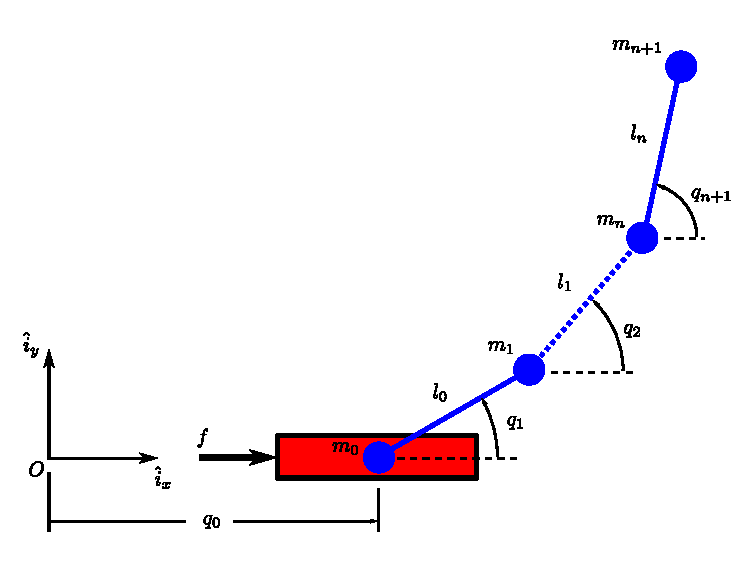
\includegraphics[width=10cm]{n-pendulum-with-cart}
\end{frame}


\begin{frame}
\frametitle{Benchmarks}
\framesubtitle{PyDy Benchmark}
\begin{table}
\begin{tabular}{l | c | c | c  }
n & SymEngine + SymPy & SymPy only & Speedup\\
\hline \hline
10 & 0.10 s & 4.42 s & 40.24x \\
15 & 0.26 s & 14.83 s & 55.95x \\
20 & 0.54 s & 36.17 s & 66.85x \\
30 & 1.60 s & 131.87 s & 82.62x \\
40 & 3.52 s & 347.11 s & 98.61x \\
50 & 6.73 s & 756.88 s & 112.46x \\
60 & 11.56 s & 1671.17 s & 114.56x
\end{tabular}
\caption{Results}
\end{table}
\end{frame}


\begin{frame}
\frametitle{Benchmarks}
\framesubtitle{PyDy Benchmark}
\includegraphics[width=10cm]{pydy}
\end{frame}


\begin{frame}
\frametitle{Summary}
\begin{itemize}
 \item SymEngine aims to be the fastest C++ symbolic manipulation library
 \item Thin wrappers to other languages (Python, Ruby, Julia, C and Haskell)
 \item Easily usable as an optional backend in SymPy, Sage and PyDy
\end{itemize}
\end{frame}


\begin{frame}
\frametitle{}
{\Large\bf Thank You}
\medskip

GitHub:
\begin{itemize}
\item \href{https://github.com/symengine/symengine}{https://github.com/symengine/symengine}
\item \href{https://github.com/symengine/symengine.py}{https://github.com/symengine/symengine.py}
\item \href{https://github.com/symengine/symengine.rb}{https://github.com/symengine/symengine.rb}
\item \href{https://github.com/symengine/symengine.jl}{https://github.com/symengine/symengine.jl}
\item \href{https://github.com/symengine/symengine.hs}{https://github.com/symengine/symengine.hs}
\end{itemize}
Mailinglist:
\begin{itemize}
\item \href{http://groups.google.com/group/symengine}{http://groups.google.com/group/symengine}
\end{itemize}
Gitter:
\begin{itemize}
\item \href{https://gitter.im/symengine/symengine}{https://gitter.im/symengine/symengine}
\end{itemize}
\end{frame}

\end{document}
